\documentclass[aspectratio=169,11pt]{beamer}

% ============================================================
% PACKAGES
% ============================================================
\usepackage{graphicx}
\usepackage{tikz}
\usetikzlibrary{positioning,arrows.meta}
\usepackage{xcolor}
\usepackage{booktabs}
\usepackage{tabularx}
\usepackage{array}
\usepackage{ragged2e}
\usepackage{hyperref}

% ============================================================
% COLORS - SAME AS PHASE-I / PHASE-II
% ============================================================
\definecolor{GEUBlue}{RGB}{20,55,105}
\definecolor{GEULightBlue}{RGB}{238,244,251}
\definecolor{GEUGrey}{RGB}{90,90,90}
\definecolor{GEULightGrey}{RGB}{245,246,248}

% ============================================================
% BEAMER SETTINGS
% ============================================================
\usetheme{default}
\setbeamertemplate{navigation symbols}{}
\setbeamertemplate{blocks}[rounded][shadow=false]

\setbeamercolor{normal text}{fg=black,bg=white}
\setbeamercolor{frametitle}{fg=GEUBlue}
\setbeamercolor{structure}{fg=GEUBlue}
\setbeamercolor{block title}{fg=GEUBlue,bg=GEULightBlue}
\setbeamercolor{block body}{fg=black,bg=GEULightBlue}

\setbeamerfont{frametitle}{size=\Large,series=\bfseries}

% ============================================================
% LOGO  (upload graphicera_logo.png to Overleaf)
% ============================================================
\newcommand{\GEULogo}{graphicera_logo.png}

% ============================================================
% HEADER
% ============================================================
\setbeamertemplate{headline}{%
  \begin{tikzpicture}[remember picture,overlay]
    \node[
        anchor=north east,
        xshift=-0.30cm,
        yshift=-0.12cm
    ] at (current page.north east)
    {\includegraphics[height=0.62cm]{\GEULogo}};
  \end{tikzpicture}
  \vspace{0.72cm}
}

% ============================================================
% FRAME TITLE
% ============================================================
\setbeamertemplate{frametitle}{%
  \vspace{0.03cm}
  \insertframetitle\par
  \vspace{0.04cm}
  \textcolor{GEUBlue}{\rule{\textwidth}{0.9pt}}
  \vspace{0.03cm}
}

% ============================================================
% FOOTER
% ============================================================
\setbeamertemplate{footline}{%
  \leavevmode
  \hbox{%
  \begin{beamercolorbox}[
      wd=.82\paperwidth,
      ht=0.32cm,
      dp=0.10cm,
      leftskip=.3cm
  ]{author in head/foot}
    \tiny Department of Computer Science \& Engineering |
    Graphic Era (Deemed to be University)
  \end{beamercolorbox}%
  \begin{beamercolorbox}[
      wd=.18\paperwidth,
      ht=0.32cm,
      dp=0.10cm,
      rightskip=.3cm
  ]{date in head/foot}
    \hfill\tiny\insertframenumber/\inserttotalframenumber
  \end{beamercolorbox}}
}

% ============================================================
% CUSTOM COMMANDS
% ============================================================
\newcommand{\smallnote}[1]{%
\vspace{0.08cm}
{\scriptsize\color{GEUGrey}#1}
}

\newcommand{\placeholder}[1]{%
\textit{\color{GEUGrey}#1}
}

% Inserts a screenshot if the file exists, otherwise shows a grey note
\newcommand{\shot}[2]{%
\IfFileExists{#1}%
{\includegraphics[width=\linewidth,height=#2,keepaspectratio]{#1}}%
{\placeholder{Insert screenshot: #1}}%
}

% ============================================================
% DOCUMENT INFORMATION
% ============================================================
\title{\textbf{Project-Based Learning}\\[2mm]\large Phase-III Evaluation}

\author{
\textbf{ExamSync -- Smart Examination Coordination Portal}\\
Team ID: DSCPP-III-2026-T079
}

\institute{
Department of Computer Science \& Engineering\\
Graphic Era (Deemed to be University), Dehradun
}

\date{Academic Session 2026--27}

% ============================================================
% DOCUMENT
% ============================================================
\begin{document}

% ============================================================
% SLIDE 1
% ============================================================
\begin{frame}[plain]

\begin{tikzpicture}[remember picture,overlay]

\draw[GEUBlue,line width=3pt]
(current page.north west) -- (current page.north east);

\node[
    anchor=north east,
    xshift=-0.45cm,
    yshift=-0.35cm
] at (current page.north east)
{\includegraphics[height=1.0cm]{\GEULogo}};

\node[
    align=center,
    text width=.84\paperwidth
] at ([yshift=.25cm]current page.center)
{
{\color{GEUBlue}
\fontsize{26}{30}\selectfont
\bfseries PROJECT-BASED LEARNING}
\\[3mm]

{\fontsize{18}{22}\selectfont
PHASE-III FINAL EVALUATION}
\\[7mm]

{\color{GEUGrey}
\Large\bfseries
ExamSync -- Smart Examination Coordination Portal}
\\[3mm]

{\color{GEUBlue}
\normalsize Team Code Quartet \quad|\quad Team ID: DSCPP-III-2026-T079}
};

\node[
    align=center,
    anchor=south,
    yshift=.42cm
] at (current page.south)
{
\bfseries
Department of Computer Science \& Engineering\\
Graphic Era (Deemed to be University), Dehradun\\[-1mm]
\scriptsize Academic Session 2026--27
};

\end{tikzpicture}

\end{frame}

% ============================================================
% SLIDE 2
% ============================================================
\begin{frame}{Team \& Mentor Details}

\begin{columns}[T,totalwidth=\textwidth]

\column{.48\textwidth}

\begin{block}{Team Information}
\begin{tabular}{@{}ll@{}}
\textbf{Team Name:} & Code Quartet\\
\textbf{Team ID:} & DSCPP-III-2026-T079\\
\textbf{Semester:} & 3rd\\
\textbf{Domain:} & Data Structures \& OOPs
\end{tabular}
\end{block}

\column{.48\textwidth}

\begin{block}{Team Members}
\small
1.\quad Shreeya Sharma (Lead) -- 2510011488\\
2.\quad Inakshi Bahukhandi -- 2512520002\\
3.\quad Rincy -- 2510010306\\
4.\quad Saumya Jha -- 2510011508
\end{block}

\end{columns}

\vspace{2mm}

\begin{block}{Mentor}
Kanishka Bhatt
\hfill
\textbf{Interactions:} 3
\end{block}

\end{frame}

% ============================================================
% SLIDE 3
% ============================================================
\begin{frame}{Project Abstract \& Problem Statement}

\begin{block}{Project Abstract}
\footnotesize
ExamSync is an examination coordination portal. A student enters a roll number
and instantly sees their room, row and seat -- no searching through seating PDFs.
It builds conflict-free seating grids, faculty invigilation rosters and records
Unfair Means (UFM) cases digitally, using C++ (DSA + OOP) with MongoDB.
\end{block}

\vspace{0mm}

\begin{block}{Problem Statement}
\footnotesize
Seating plans come as long PDFs, so students waste time finding their seat, and
manual seating and duty planning leads to clashes and same-branch students
sitting together.
\end{block}

\vspace{-1.5mm}

\textbf{\color{GEUBlue}Target Users / Application}

\begin{itemize}\itemsep1pt
    \footnotesize
    \item Students, teachers / invigilators and the examination admin
    \item University exam cell -- many exams running across different blocks
    \item Faster seat lookup, fewer clashes, paperless UFM records
\end{itemize}

\end{frame}

% ============================================================
% SLIDE 4
% ============================================================
\begin{frame}{Objectives \& Final Deliverables}

\begin{columns}[T,totalwidth=\textwidth]

\column{.48\textwidth}

\textbf{\color{GEUBlue}Finalized Objectives}

\begin{enumerate}\itemsep3pt
    \small
    \item Instant seat lookup using a roll number
    \item Conflict-free seating (no same-branch neighbours)
    \item Handle room capacity and multiple simultaneous exams
    \item Fair invigilation roster with no double booking
    \item Digital UFM logging with separate role-based logins
\end{enumerate}

\column{.48\textwidth}

\textbf{\color{GEUBlue}Final Deliverables}

\begin{itemize}\itemsep3pt
    \small
    \item Automated seating allocation engine (C++)
    \item Student, teacher and admin portals
    \item Teacher duty allocation module
    \item Digital UFM logger with admin review
    \item MongoDB sync + CSV dataset and source code
\end{itemize}

\end{columns}

\vfill

\smallnote{
Every objective on the left maps to one deliverable on the right.
}

\end{frame}

% ============================================================
% SLIDE 5  (Phase-II feedback only)
% ============================================================
\begin{frame}{Phase-II Feedback Incorporated}

\scriptsize

\begin{center}

\renewcommand{\arraystretch}{1.35}

\begin{tabularx}{.96\textwidth}
{@{}p{5.6cm}X@{}}

\toprule
\textbf{Feedback / Suggestion} &
\textbf{Action Taken}\\
\midrule

Student CSV data was not yet connected to MongoDB &
Student data imported and synced with MongoDB\\

Database module was only partly complete (80\%) &
Database \& sync finished (100\%), with batched writes\\

\bottomrule

\end{tabularx}

\end{center}

\vfill

\begin{block}{Final Improvement}
\small
The project moved from a basic seating idea to a complete system: roll lookup,
multi-exam allocation, duty rostering, digital UFM logging and three
role-based portals, all backed by MongoDB.
\end{block}

\end{frame}

% ============================================================
% SLIDE 6
% ============================================================
\begin{frame}{Final System Architecture}

\begin{center}

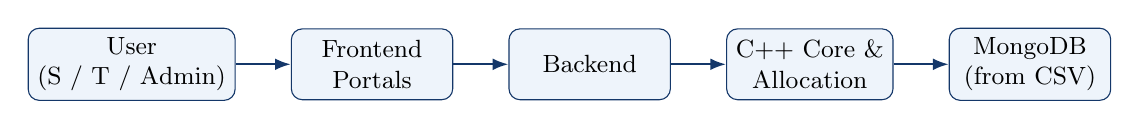
\begin{tikzpicture}[
node distance=7mm,
box/.style={
rectangle,
rounded corners,
draw=GEUBlue,
fill=GEULightBlue,
minimum width=2.05cm,
minimum height=9mm,
align=center,
font=\small
},
arrow/.style={
-{Latex[length=2mm]},
thick,
draw=GEUBlue
}
]

\node[box] (a) {User\\(S / T / Admin)};
\node[box,right=of a] (b) {Frontend\\Portals};
\node[box,right=of b] (c) {Backend};
\node[box,right=of c] (d) {C++ Core \&\\Allocation};
\node[box,right=of d] (e) {MongoDB\\(from CSV)};

\draw[arrow] (a)--(b);
\draw[arrow] (b)--(c);
\draw[arrow] (c)--(d);
\draw[arrow] (d)--(e);

\end{tikzpicture}

\end{center}

\vspace{4mm}

\begin{columns}[T,totalwidth=\textwidth]

\column{.48\textwidth}

\textbf{\color{GEUBlue}Major Components}

\begin{itemize}\itemsep2pt
    \small
    \item Core layer: OOP classes + hash-based roll index
    \item Allocation layer: seating constraints, overflow
    \item Data layer: CSV import + MongoDB sync
    \item Backend + role-based frontend portals
\end{itemize}

\column{.48\textwidth}

\textbf{\color{GEUBlue}System Flow}

\begin{itemize}\itemsep2pt
    \small
    \item Input: CSV data and portal requests
    \item Processing: seat grids, duty roster
    \item Storage: MongoDB collections
    \item Output: seat details, duties, UFM status
\end{itemize}

\end{columns}

\end{frame}

% ============================================================
% SLIDE 7
% ============================================================
\begin{frame}{Final Technology Stack}

\begin{columns}[T,totalwidth=\textwidth]

\column{.48\textwidth}

\begin{block}{Software / Technologies}
\begin{itemize}\itemsep2pt
    \small
    \item Language: C++ (OOP)
    \item Data structures: hash map, 2D vector grids
    \item Algorithm: graph-coloring backtracking
    \item Database: MongoDB
    \item Data input: CSV files
    \item Communication: HTTP-based backend
\end{itemize}
\end{block}

\column{.48\textwidth}

\begin{block}{Development Infrastructure}
\begin{itemize}\itemsep2pt
    \small
    \item Version Control: Git / GitHub
    \item Repository: inakshi17/ExamSync
    \item Testing: unit, constraint, stress, integration and duty tests
    \item Documentation: Overleaf (LaTeX) report and slides
\end{itemize}
\end{block}

\end{columns}

\vfill

\smallnote{
MongoDB is used for storage throughout the project.
}

\end{frame}

% ============================================================
% SLIDE 8
% ============================================================
\begin{frame}{Implementation of PBL Course Concepts}

\scriptsize

\begin{center}

\renewcommand{\arraystretch}{1.4}

\begin{tabularx}{.96\textwidth}
{@{}>{\bfseries}p{2.8cm}X p{3.2cm}@{}}

\toprule
Course & Concepts Actually Implemented & Project Module\\
\midrule

Data Structures in C &
Hash map for O(1) roll lookup, 2D vector grids for rooms,
graph-coloring backtracking for seating constraints &
Seating engine, roll lookup\\

OOPs with C++ &
Classes for users, students, teachers, rooms, seating and UFM records;
encapsulation; STL containers &
Core layer, UFM logger\\

\bottomrule

\end{tabularx}

\end{center}

\end{frame}

% ============================================================
% SLIDE 9
% ============================================================
\begin{frame}{Module-Wise Final Implementation}

\scriptsize

\begin{center}

\renewcommand{\arraystretch}{1.0}

\begin{tabularx}{.96\textwidth}
{@{}p{2.7cm}X p{2.5cm}p{1.5cm}@{}}

\toprule
\textbf{Module} &
\textbf{Implementation} &
\textbf{Responsible} &
\textbf{Status}\\
\midrule

Seating Engine &
Conflict-free grids, multi-exam allocation, capacity and overflow handling &
Shreeya, Inakshi &
Completed\\

Duty Allocation &
Invigilation scheduling, duty distribution, double-booking checks &
Shreeya, Inakshi &
Completed\\

Role-Based Portals &
Student, teacher and admin logins, navigation and interface &
Rincy &
Completed\\

Seating Visualization &
Room-wise seating grid view and date-wise seating display in the portals &
Rincy &
Completed\\

UFM Module &
Digital UFM logger, record storage, admin review workflow &
Saumya &
Completed\\

Database \& Infra &
CSV import, MongoDB sync, project integration &
Saumya &
Completed\\

\bottomrule

\end{tabularx}

\end{center}

\vspace{0mm}

\begin{center}
\colorbox{GEULightBlue}{
\parbox{.65\textwidth}{
\centering
\textbf{Final Project Completion:} 100\%
}}
\end{center}

\end{frame}

% ============================================================
% SLIDE 10
% ============================================================
\begin{frame}{Working System / Prototype Demonstration}

\begin{columns}[T,totalwidth=\textwidth]

\column{.43\textwidth}

\textbf{\color{GEUBlue}Major Working Features}

\begin{itemize}\itemsep3pt
    \small
    \item Roll number $\rightarrow$ room, floor, row, seat
    \item Conflict-free seating grids
    \item Teacher duty and flying squad dashboard
    \item Digital UFM logging with live status
    \item Admin console to load data and manage exams
\end{itemize}

\column{.53\textwidth}

\begin{block}{System Screenshot / Output}

\centering
\vspace{2mm}

\shot{admin_portal.png}{3.6cm}

\vspace{2mm}

\end{block}

\end{columns}

\vfill

\smallnote{
Live demo will be shown during the evaluation; the screenshot is only for support.
}

\end{frame}

% ============================================================
% SLIDE 11
% ============================================================
\begin{frame}{Data / Database / Backend Implementation}

\begin{columns}[T,totalwidth=\textwidth]

\column{.48\textwidth}

\textbf{\color{GEUBlue}Data / Database}

\begin{itemize}\itemsep3pt
    \small
    \item Source: CSV files (students, rooms, faculty, schedules)
    \item Storage: MongoDB, synced from C++ structures
    \item Entities: users, students, teachers, rooms, seating, UFM
    \item Retrieval: hash-based index for roll numbers
    \item Sync: CSV loaded once at startup, batched writes
\end{itemize}

\column{.48\textwidth}

\textbf{\color{GEUBlue}Backend / Core Logic}

\begin{itemize}\itemsep3pt
    \small
    \item Core: OOP classes managing rooms and seating
    \item Service: HTTP calls for seats, duties and UFM
    \item Logic: backtracking to avoid same-branch neighbours
    \item Overflow: extra students move to nearby rooms
    \item Security: centralised role checks for each portal
\end{itemize}

\end{columns}

\end{frame}

% ============================================================
% SLIDE 12
% ============================================================
\begin{frame}{Testing \& Validation}

\scriptsize

\begin{center}

\renewcommand{\arraystretch}{1.25}

\begin{tabularx}{.96\textwidth}
{@{}p{2.2cm}p{2.5cm}X p{0.9cm}@{}}

\toprule
Test Type &
Tested &
Observed Result &
Status\\
\midrule

Unit Test &
Roll number lookup &
O(1) lookup validated across all records &
Pass\\

Constraint Test &
Branch non-collision &
0 adjacent or diagonal violations in generated grids &
Pass\\

Stress Test &
Multi-exam allocation &
Simultaneous exams across blocks, no room overflow &
Pass\\

Integration Test &
UFM entry and DB sync &
UFM logs update live in MongoDB with faculty ID and status &
Pass\\

Duty Test &
Invigilation roster &
No teacher double-booked in the generated roster &
Pass\\

\bottomrule

\end{tabularx}

\end{center}

\vspace{2mm}

\begin{block}{Validation Summary}
\small
All five test groups passed against the project objectives.
\end{block}

\end{frame}

% ============================================================
% SLIDE 13
% ============================================================
\begin{frame}{Results \& Performance Analysis}

\begin{columns}[T,totalwidth=\textwidth]

\column{.48\textwidth}

\textbf{\color{GEUBlue}Key Results}

\begin{itemize}\itemsep3pt
    \small
    \item O(1) seat lookup by roll number
    \item 0 adjacent / diagonal same-branch violations
    \item No room overflow with simultaneous exams
    \item No teacher double-booked
\end{itemize}

\column{.48\textwidth}

\begin{block}{Data Handled by the System}

\centering
\renewcommand{\arraystretch}{1.3}
\begin{tabular}{@{}lr@{}}
\textbf{Students} & 20,045\\
\textbf{Exam halls} & 67 (4,917 seats)\\
\textbf{Faculty} & 500\\
\textbf{Exam schedule records} & 7,078
\end{tabular}

\end{block}

\end{columns}

\end{frame}

% ============================================================
% SLIDE 14
% ============================================================
\begin{frame}{GitHub Repository \& Development Evidence}

\begin{columns}[T,totalwidth=\textwidth]

\column{.50\textwidth}

\textbf{\color{GEUBlue}Repository Details}

\begin{itemize}\itemsep3pt
    \small
    \item Main repo: {\scriptsize\url{github.com/inakshi17/ExamSync}}
    \item Phase-III folder: {\scriptsize\texttt{PHASE-3}}
    \item Branch: main
    \item Contributors: all 4 team members
\end{itemize}

\column{.46\textwidth}

\textbf{\color{GEUBlue}Key Commits}

\begin{itemize}\itemsep3pt
    \small
    \item \texttt{XX} -- backend folder
    \item \texttt{XX} -- dataset folder
    \item \texttt{XX} -- dsa folder
    \item \texttt{XX} -- frontend folder
\end{itemize}

\end{columns}

\vfill

\smallnote{
Full commit history and each member's individual commits are visible on GitHub.
}

\end{frame}

% ============================================================
% SLIDE 15
% ============================================================
\begin{frame}{Individual Contribution}

\scriptsize

\begin{center}

\renewcommand{\arraystretch}{1.25}

\begin{tabularx}{.96\textwidth}
{@{}p{1.9cm}>{\RaggedRight\arraybackslash}p{2.1cm}X p{1.3cm}@{}}

\toprule
Member &
Role &
Final Technical Contribution &
Commits\\
\midrule

Shreeya Sharma &
DSA / Core (Lead) &
Tuned seating for multiple simultaneous exams across blocks; finalised duty allocation and invigilation scheduling &
XX\\

Inakshi Bahukhandi &
DSA / Core &
Fixed constraint-checking and overflow handling; added double-booking checks for teacher duties &
XX\\

Rincy &
Frontend \& OOP &
Improved navigation across student, teacher and admin portals; refined the interface and finished the OOP class set &
XX\\

Saumya Jha &
Backend \& Docs &
Completed MongoDB sync between memory structures and database; finished digital UFM logger and admin review &
XX\\

\bottomrule

\end{tabularx}

\end{center}

\end{frame}

% ============================================================
% SLIDE 16
% ============================================================
\begin{frame}{Challenges, Limitations \& Lessons Learned}

\begin{columns}[T,totalwidth=\textwidth]

\column{.52\textwidth}

\textbf{\color{GEUBlue}Challenges \& Solutions}

\begin{itemize}\itemsep2pt
    \scriptsize
    \item Clashes in shared rooms with simultaneous exams -- now tracked per exam slot, per room
    \item Same-branch students seated diagonally at corners and row ends -- neighbour checks rewritten and re-tested
    \item Slow MongoDB sync for large data -- batched writes, CSV loaded once
    \item Wrong role redirects in portals -- role checks centralised
\end{itemize}

\vspace{2mm}

\textbf{\color{GEUBlue}Current Limitations}

\begin{itemize}\itemsep2pt
    \scriptsize
    \item Seating rules cover branch / subject neighbours only
    \item Data is loaded from CSV at startup
\end{itemize}

\column{.44\textwidth}

\textbf{\color{GEUBlue}Technical Learning}

\begin{itemize}\itemsep3pt
    \scriptsize
    \item Using hashing and backtracking on real data
    \item Keeping in-memory C++ data in sync with MongoDB
    \item Testing edge cases on every generated grid
\end{itemize}

\vspace{2mm}

\textbf{\color{GEUBlue}Team Learning}

\begin{itemize}\itemsep2pt
    \scriptsize
    \item Working together through GitHub
    \item Splitting modules and integrating them
\end{itemize}

\end{columns}

\end{frame}

% ============================================================
% SLIDE 17
% ============================================================
\begin{frame}{Final Outcomes, Applications \& Future Scope}

\begin{columns}[T,totalwidth=\textwidth]

\column{.32\textwidth}

\textbf{\color{GEUBlue}Final Outcomes}

\begin{itemize}\itemsep3pt
    \small
    \item Automated seating system
    \item Student, teacher and admin portals
    \item Digital UFM logger
\end{itemize}

\column{.32\textwidth}

\textbf{\color{GEUBlue}Applications}

\begin{itemize}\itemsep3pt
    \small
    \item University exam cells
    \item Colleges and schools
    \item Entrance / competitive exam centres
\end{itemize}

\column{.32\textwidth}

\textbf{\color{GEUBlue}Future Scope}

\begin{itemize}\itemsep3pt
    \small
    \item Mobile app and seat notifications
    \item More seating rules
    \item Exam analytics for admin
\end{itemize}

\end{columns}

\vspace{5mm}

\begin{block}{Tangible Project Outcome}
\small
A complete working system: C++ seating and duty engine, MongoDB-backed
role-based portals and a paperless UFM logger, tested on 20,045 students and
67 exam halls.
\end{block}

\end{frame}

% ============================================================
% SLIDE 18
% ============================================================
\begin{frame}{References \& Project Resources}

\begin{columns}[T,totalwidth=\textwidth]

\column{.56\textwidth}

\textbf{\color{GEUBlue}References}

\begin{enumerate}\itemsep3pt
    \scriptsize
    \item Ayeesha Begum S, et al. \textit{Algorithm Based Seating Arrangement System}, IJFMR.
    \item Asif A, et al. \textit{Smart Exam Management Platform}, IJRTI.
    \item Herbert Schildt, \textit{C++: The Complete Reference}, McGraw Hill.
    \item MongoDB documentation -- docs.mongodb.com
\end{enumerate}

\column{.40\textwidth}

\textbf{\color{GEUBlue}Project Resources}

\begin{itemize}\itemsep3pt
    \small
    \item GitHub: {\scriptsize github.com/inakshi17/ExamSync}
    \item Demo: live during evaluation
\end{itemize}

\vfill

\begin{center}

\colorbox{GEUBlue}{
\parbox{.82\textwidth}{
\centering
\color{white}
\Large\textbf{Thank You}
}}

\end{center}

\end{columns}

\end{frame}

\end{document}
